\documentclass{llncs}

%\usepackage{makeidx}  % allows for indexgeneration
\usepackage{graphicx}

\begin{document}

\title{SWAML, from Mailing Lists to the Semantic Web}

\titlerunning{SWAML, from Mailing Lists to the Semantic Web}

\author{
Sergio Fern\'andez \and Diego Berrueta \and Jose E. Labra
}

\authorrunning{Sergio Fern\'andez et al.}

\tocauthor{Sergio Fern\'andez, Diego Berrueta, Jose E. Labra (Universidad de Oviedo)} 

\institute{Universidad de Oviedo, \\
Technical School of Computer Science, \\
Oviedo, Asturias, Spain,\\
\email{sergio@wikier.org, diego@berrueta.net, labra@uniovi.es},\\
WWW home page: \texttt{http://swaml.berlios.de/}
}

\date{1 February 2007}

\maketitle

\begin{abstract}

Mailing list archives (i.e., the messages posted up-to-now) are often published 
on the web and indexed by conventional search engines. They store a vast 
knowledge capital. However, the ability to auto-matically recognize and process 
the information is mostly lost at publishing time. As a result, the current 
mailing list archives are hard to query and have a limited use. This paper 
describes how SWAML uses Semantic Web technologies in order to avoid the
information loss and to allow new applications able to exploit this 
information in a more convenient way.

\end{abstract}

\section{Introduction}

The electronic mail is one of the best tools that Internet has. Using the
email persons exchange information at his job and with his friends. A big 
percent of mail traffic involves mail lists. Mail lists is a dicussion forum,
allowing users to discuss different topics with people who shares his interests.
All these discussions and arguments (including sometimes experts "interventions") 
are logged and stored, and suposse a big knowledge database. Often the mailing 
list archives are published in tradicional formats, like HTML. But, although 
these formats allow to have the information available to index, it loses a lot 
of information about the relationships between the messages.

Then it's necessary to publish these old archives into a much rich format\cite{Luke2004}.
A format that mainly fulfills 2 intentions:
\begin{itemize}
  \item Publish the archives with the smaller possible loss of information,
	about the author, the messages in the thread, etc.
  \item Allow to refer this information for external uses.
\end{itemize}

\subsection{SIOC}

SIOC (Semantically-Interlinked Online Communities) provides methods for 
interconnecting discussion methods such as blogs, forums and mailing lists 
to each other. It consists of the SIOC ontology, an open-standard machine 
readable format for expressing the information contained both explicitly 
and implicitly in internet discussion methods, of SIOC metadata producers 
for a number of popular blogging platforms and content management systems, 
and of storage and browsing/searching systems for leveraging this SIOC 
data. \cite{Breslin2005}

The goal of SIOC \footnote{\url{http://sioc-project.org/}} is to interconnect
these online communities. Community sites can include many discussion primitives,
such as bulletin boards, weblogs and mailing lists, which it have grouped under 
the concept of forum.

%\begin{figure}[ht]
% \centering
% 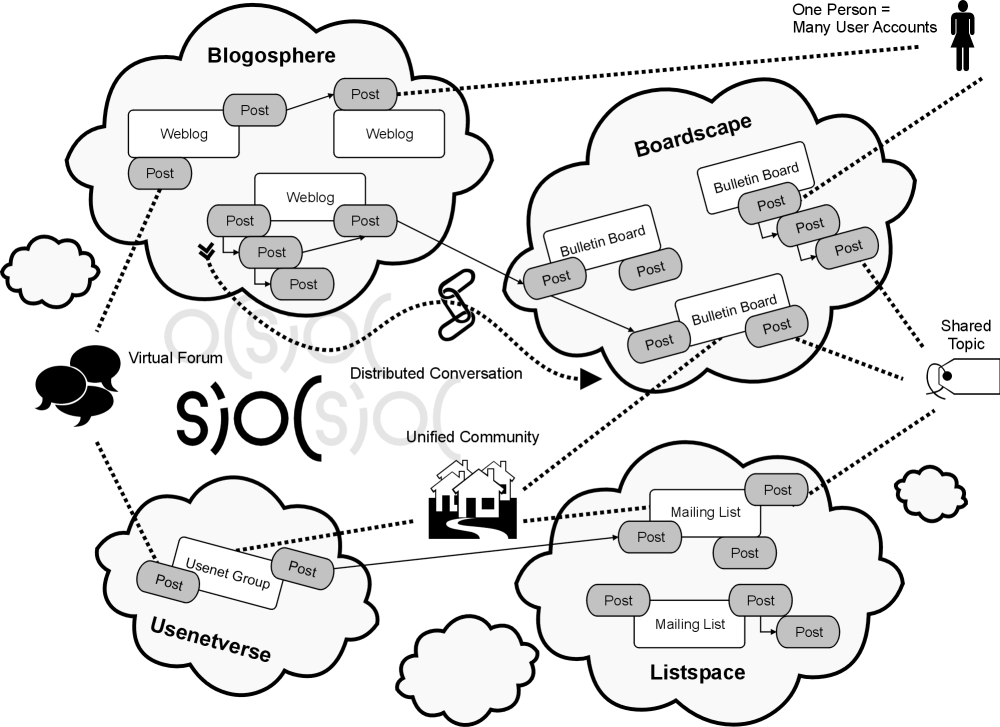
\includegraphics[bb=0 0 240 174]{images/sioc-discussion.png}
% \caption{Connections between discussion clouds with SIOC}
%\end{figure}

FIXME: add a graphic about relations between forums

Then \texttt{Forum} class is the most important for us at SIOC ontology. In the 
domain of a forum there are another classes at the ontology, mainly we need two
of it: \texttt{Post} and \texttt{User} 

The SIOC community has developed several wrappers that allows to export instances
of community site concepts (such as blogs o forums) in RDF format. But the effort 
is only centered in providing mappings from web-based systems, forgetting all the 
knowledgement stored in a large number of legacy systems preceding the current Web.

\section{Formal model}

FIXME (talk with Polo)

\section{Components}

In the SWAML project are involved several components, mainly three:

\begin{itemize}
 \item SWAML, the core process that exports a mailing list in RDF.
 \item Buxon, a browser for SIOC Forum instances.
 \item SWAML Ontology.
\end{itemize}

Each of it each one fulfills a concrete purpose into the global purposes that 
the project persecutes. The project covers so much the data exportation phase 
as the data consumition phase.

\subsection{SWAML}

The main component, the core, is called with the same name that the project. SWAML is
the process in charge to process the mailing lists . SWAML reads a collection of email 
messages stored in a mailbox (from a mailing list compatible with RFC 4155) and generates 
a RDF description. It is written in Python using SIOC as the main ontology to represent 
in RDF a mailing list.

\begin{figure}[ht]
 \centering
 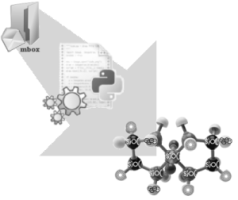
\includegraphics[bb=0 0 238 200]{images/swaml-process.png}
 \caption{SWAML core process}
\end{figure}

The SWAML project fulfills a much-needed requirement for the Semantic Web: to be able 
to refer to semantic versions of email messages and their properties using a resource 
URI. By reusing the SIOC vocabulary for describing online discussions, SWAML allows 
users of SIOC to refer to email messages from other discussions taking place on forums, 
blogs, etc., so that distributed conversations can occur across these discussion media. 
Also, by providing email messages in SIOC format, SWAML are providing a rich source of 
data, namely mailing lists, for use in SIOC applications. 

\subsection{Buxon}

Buxon is the application that make the opposite work. It takes the URI of a generic SIOC 
Forum (for example a mailing list exported by SWAML, although it's independent of the 
export tool) and it recompose the graph. With that graph the tool shows the posts ordered 
by threads using a similar GUI than the classic mail clients.

\begin{figure}[ht]
 \centering
 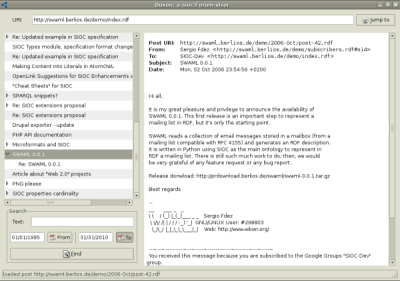
\includegraphics[bb=0 0 288 202]{images/buxon.png}
 \caption{Buxon in action (FIXME: add a screenshot of v0.0.4)}
\end{figure}

In addition it allows to make simple searches by terms and dates over the back-end graph.

FIXME: support to PingTheSemanticWeb.com (search a cite)

\subsection{SWAML Ontology}

Until SIOC ontology contemplates some subclasses of Forum, it's necessary 
to add some properties. Concretely in version 0.2 of our ontology 
\footnote{http://swaml.berlios.de/ns/0.2} we have reduced these properties 
to only two:

\begin{itemize}
  \item \texttt{previousByDate} to link with the previous post sent in the 
	mailing list..
  \item \texttt{nextByDate} to link with the post that was sent after by date 
	in the mailing list.
\end{itemize}

Both under the domain and the range of \texttt{sioc:Post}. Perhaps these 
properties has a minor importance to describe generic forums instances, 
but its meaning receives greater importance in the concrete scope of a 
mailing list.

\section{Conclussions and Future Work}

FIXME, interesting stuff here... (conclussions)

We are exploring some directions for future work. Some of them are:

\begin{itemize}
  \item Integration of the SWAML process with a popular HTML-based
        mailing list archiver, such as Hypermail or Pipermail, would be
        a gigant push to speed up the adoption of SWAML. It is well
        known that one of the most awkward problems of any technology
        is to gain a critical mass of users. The semantic web is not
        an exception. A good recipe to tackle this problem is to
        integrate the new technologies into old tools, making
        a smooth transition without requiring any extra effort from
        the users. Merging the SWAML process into the batch flow of
        tools such as Hypermail would allow to generate both
        HTML and RDF versions of the archive. Those could reside
        side-by-side on the web server, even sharing the same URI
        by means of content-negotiation~\cite{Recipes}.
  \item Actually, integration could be pushed further away through
        RDFa~\cite{Birbeck2006}, embedding the RDF content into the
        XHTML documents.
  \item So far, no semantic annotation relative to the meaning of
        the messages is considered. Obviously, this information can not
        be derived from a RFC 4155-compilant mailbox. However, it is
        conceivable that it can be added by other means, for instance,
        by social tagging using folksonomies, or by parsing the RDFa
        that can exist in the messages that are send in XHTML format.
  \item The metadata extracted from a mailing list archive can be
        quite huge. Even after removing the body of the messages, the
        XML/RDF metadata of a mailing list containing 1000 messages may
        have a size of ??? KBytes, with a linear growth. It is not uncommon
        for a busy mailing list to generate this volume of messages
        monthly. Hence, it is imperative to design a mechanism to
        fragmentate the dataset. The SWAML process splits each message
        in a separate RDF document, but this arbitrary decision clearly
        does not fit every application. A much better solution would be to
        create an easy-to-deploy SPARQL endpoint\cite{SPARQL},
        that translates the
        decision on how to partition the data to the final application.
  \item To make agile the obtaining of several mailboxes:
	To improve the experiment done using LibGmail
	
	the simplest form to obtain a lot of mail lists is to serializar to mboxes 
	the posts stored by the users in its mail accounts. The preliminar experiment 
	was made across a GMail account subscribed to a semantic web related mailing list
	\footnote{\url{http://www.johnbreslin.com/blog/2006/11/08/buxon-visor-for-siocforum-browsing/}},
	but 
  \item Integration with Mailman.
\end{itemize}

%\section{Acknowledgements}
%
%The authors would like to express their gratitude to Dr. John Breslin and
%Uldis Bojars, whose support and contributions have been of great help
%to this project.

\bibliographystyle{abbrv}
\bibliography{../references}
%
\end{document}
